%%%%%%%%%%%%%%%%%%%%%%%%%%%%%%%%%%%%%%%%%%%%%%%%%%%%%%%%%%%%%%%%%%%%%%%%%%%%%%%%%%%%%%
% author                : louis tomczyk
% date of production    : 2024-02-11
% licence               : cc-by-nc-sa
%                         Attribution - Non-Commercial - Share Alike 4.0 International
%%%%%%%%%%%%%%%%%%%%%%%%%%%%%%%%%%%%%%%%%%%%%%%%%%%%%%%%%%%%%%%%%%%%%%%%%%%%%%%%%%%%%%

\bfig
    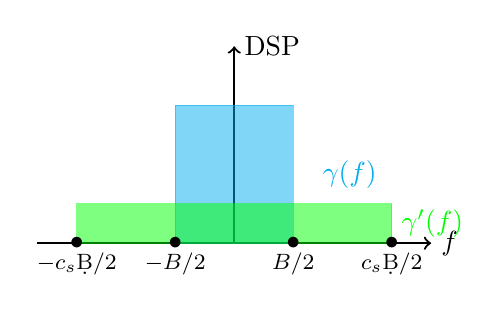
\begin{tikzpicture}[scale = 0.5]
        \draw[->,thick] (0,0) --++ (10,0) node[right]{$f$};
        \draw[->,thick] (5,0) --++ (0,5) node[right]{DSP};

        \draw[fill = cyan, color = cyan, opacity = 0.5] (3.5,0) rectangle (6.5,3.5)
        node[midway,right = 1cm, opacity =1]{$\gamma(f)$};
        \draw[fill = green, color = green, opacity = 0.5] (1,0) rectangle (9,1)
        node[midway,right = 2cm, opacity =1]{$\gamma'(f)$};

        \draw (3.5,0) node{$\bullet$}node[below]{\footnotesize $-B/2$};
        \draw (6.5,0) node{$\bullet$}node[below]{\footnotesize $B/2$};

        \draw (1,0) node{$\bullet$}node[below]{\footnotesize $-c_s\d B/2$};
        \draw (9,0) node{$\bullet$}node[below]{\footnotesize $c_s\d B/2$};
    \end{tikzpicture}
    \caption{Illustration de l'étalement du bruit induit par un sur-échantillonnage
    de facteur $c_s>2$.}
    \label{fig:EtalementSurechantillonage}
\efig